% LaTeX .tex example for the proceedings of
% COBEM 2015 - 23rd International Congress of Mechanical Engineering
% November, 6-11 2015 - Rio de Janeiro, RJ, Brazil
%
% Based on the template of the proceedings of COBEM2013 
%
% Max. 8 pg

\pdfminorversion=4
\pdfobjcompresslevel=1


\documentclass[10pt,fleqn,a4paper,twoside]{article}
\usepackage{cobem2015}

\usepackage{amsmath}
\usepackage{todonotes}
\graphicspath{ {./Figs/} }

\usepackage{subfigure}

\def\shortauthor{R. Corsi, J. Jaime}
\def\shorttitle{Active Magnetic Bearing Project For a Satellite Reaction Wheel}

\newcommand{\executeiffilenewer}[3]{%
	\ifnum\pdfstrcmp{\pdffilemoddate{#1}}%
	{\pdffilemoddate{#2}}>0%
	{\immediate\write18{#3}}\fi%
}

\newcommand{\includesvg}[1]{%
	\executeiffilenewer{#1.svg}{#1.pdf}%
	{inkscape -z -D --file=./Figs/#1.svg %
		--export-pdf=./Figs/#1.pdf --export-latex}%
	\input{./Figs/#1.pdf_tex}%
}


\begin{document}
	\fphead
	\hspace*{-2.5mm}\begin{tabular}{||p{\textwidth}}
		\begin{center}
			\vspace{-4mm}
			\title{ACTIVE MAGNETIC BEARING PROJECT FOR A SATELLITE REACTION WHEEL}
		\end{center}
		\authors{Rafael~Corsi~Ferr\~{a}o} \\
		\authors{Jos\'{e} Jaime da Cruz} \\
		\institution{Escola Polit\'ecnica da Cidade de S\~{a}o Paulo} \\
		\institution{corsiferrao@gmail.com, jaime@lac.usp.br} \\
		\\
		%\authors{Third Author's Name} \\
		%\institution{Institution and address for third author} \\
		%\institution{e-mail} \\
		%\\
		%\authors{Same format for others authors, if any} \\
		\\
		\abstract{\textbf{Abstract.} In this paper, the development of a novel active magnetic bearing (MB) system for reaction wheels applicable in satellite attitude control is presented. The proposed bearing has four degrees of freedom passively stable (EMB) by one pair of permanent magnet; two degrees of freedom (AMB) are actively stabilized by eight electromagnetic poles. The  magnetic model of both EMB and AMB are presented and  equations of force-current and force-position are analyzed by the magnetic circuit approach and by the finite element method. With the force characteristic curves a non-linear dynamic model for the MB and a control system that stabilizes the bearing at its operating point are presented. A flat, uncoupled and scalable magnetic bearing with good stiffness, that can be used on satellites reaction wheels to improve its performance and reliability, is obtained. A prototype is under construction. Simulation results are presented.}\\
		\\
		\keywords{\textbf{Keywords:} Magnetic Bearing, Satellite Attitude Control }\\
	\end{tabular}
	
	\section{INTRODUCTION}
	The attitude and orbit control is one of the most critical technology of any spatial systems \cite{wertz1978spacecraft}, the main actuators include propellants, magnetic torques and reaction wheels.  Reaction wheels are hard to replace because they present a large operating range in torque (unlike magnetic actuators) and are powered by renewable energy provided by solar panels (unlike propellers based on a finite fuel supply). For these reasons, reaction wheels are present on virtually any satellite with a  minimum performance requirements in attitude.
	
	A reaction wheel can be described as an inertial actuator operating on the principle of conservation of angular momentum. The performance of the reaction wheel on the satellite takes place by exchange of angular momentum, limited to the axis of rotation of the wheel. Due to the large difference between the satellite and the inertia of the reaction wheel, a control of attitude with great, precision is possible with this system.
	
	Reaction wheels typically consist of an electric motor, usually a DC brushless motor, a bearing system and one element of inertia. The inertia member and the motor are mounted on bearings to ensure precise rotation about an axis. The rotation speed of the system is controlled by an electronic motor drive. Reaction wheels can be operated in two distinct ways: by rotation or torque.
	
	The suspension of the rotor relative to the stator is a critical part in the reaction wheels \citep{taniwaki2003experimental} the consequences of any friction in the relative movement between these two components. Indeed, the friction is reflected  in a greater consumption of electric power, introduction of a dead zone of operation in torque as well as limited life of the reaction wheel due to gradual wear of the bearing.
	
	A  mechanical solution for the interface between the rotor and the stator is a rolling bearing. Despite its apparent simplicity, challenges for achieving the minimum friction values needed in view of the demands of consumption and easiness of control \citep{Krishnan2010}.
	In the case of aerospace applications, lubrication rolling is also difficulty due to the impossibility of using traditional lubricants under conditions of low or no air pressure, which leads to loss of volatile components (lubricants) and their consequent deterioration. Another difficulty is due to the trend of migration of lubricants in the absence of gravity, which is usually addressed with strategies to recapture or relubrication.
	
	Another solution is to use a magnetic bearing \citep{Bangcheng2012}, which is an alternative without mechanical contact between the rotor and the stator. The gain in reliability and lifetime of the reaction wheel is considerable \citep{Marble2006}, and basically limited by the durability of electronics. The non-contact operation eliminates the need for lubrication and consequently enables the operation under vacuum which results in simplifying the mechanical design requirements.
	
	\subsection{Magnetic Bearing for Reaction Wheel}
	
	There is in the literature three different topologies for  bearings in magnetic reaction wheels, have mostly two degrees of freedom active, and makes use of permanent magnets aiming to minimize power consumption.
	
	The topology proposed by \cite{Bernus1998} works with two active degrees of liberties having the permanent magnets on the rotor and two stators. The rotor has  "I" cross shape and it is surrounded by the external and internal stator with both "C" cross shape. The internal stator is used for active control radial directions has four independent poles to generate flux which also contributes to increase the axial stiffness of the rotor. Passive degrees of freedoms are stabilized by the magnetic flux generated by the permanent magnet.
	
	Another magnetic bearing proposition\citep{Scharfe2001} also works with the radial direction controlled, it has only one stator that is located at the center of the bearing and one external rotor, both parts have a "C" cross shape. The permanent magnetic poles are located on the rotor generating a magnetic flux that stabilizes the axial direction, this topology allows generating a subtractive magnetic flux in some parts of the rotor in favor of decrease the attraction force and places the rotor at the operation point with less effort. 
	
	A recent topology proposed by \cite{Bangcheng2012} has  three degree of freedom controlled, this magnetic bearing  provides an substantial axial stiffness (passive axis) in order to maintain the rotor on its operation point when applied to high rotor speeds.
		
	\section{Project}
	
	The magnetic bearing proposed in this work is inspired on the topologies by \cite{Bernus1998} and \cite{Scharfe2001}. The bearing has four degrees of freedom passively stable: tilt, row, pitch and its axial direction, the other two degrees of freedom (radial) are actively stabilized. Torque imposed for the rotation of the rotor is developed by an electric motor brushless DC (BLDC) placed inside the bearing. The magnetic circuit comprises two stators: one outer rotor and other inner rotor. The first one is responsible for stabilization of passives degrees of freedom and the inner one to control the rotor radial position through eight magnetic poles.% Was decided to install the permanent magnets in the external stator not in the rotor as seen in the literature, seeking to the best mechanical balance of the rotor. 
	Figure \ref{fig:mancal:corte} is a cut of the proposed bearing.
	
	We adopted a flat geometry to better stiffness in the unstable modes of the bearing. The outboard bearing to the motor enables a stiffness within the proposed limits of mass and dimensions.
	
	\begin{figure}[ht]
		\centering
		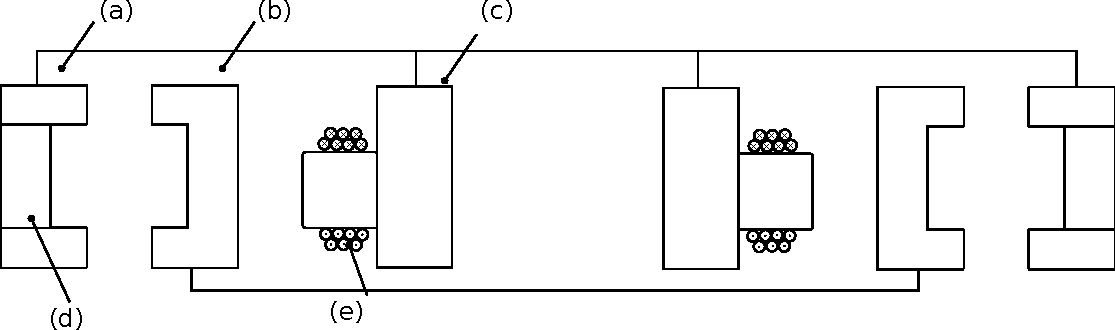
\includegraphics[width=1\linewidth]{Figs/mancais/mancal_corte2}
		\caption{Radial cut of the proposed magnetic bearing. (a) External stator; (b) Rotor; (c) Internal stator; (d) Permanent magnetics; (e) Coils}
		\label{fig:mancal:corte}
	\end{figure}
	
	\subsection{External Stator and Rotor}
	
	Magnetic circuit of a section of the outer stator is illustrated in Figure \ref{fig:circuito:passivo}. The magnetic flux generated by the permanent magnet seeks the path of the least reluctance to close the magnetic circuit. This occurs by way of the external stator irons ($\mathcal{R}_f$), then passing through the air gap ($\mathcal{R}_g$) and rotor ($\mathcal{R}_{fr}$). The permanent magnetic is a magnetic field source and is located between two irons. 
	The rotor undergoes attraction on all direction, at equilibrium (with a symmetrical air gap) the resultant force would tend to be null and remain in equilibrium at the operating point (critically stable). 
			
	\begin{figure}[ht]
		\subfigure[Magnetic circuit of the outer stator and rotor]{	
			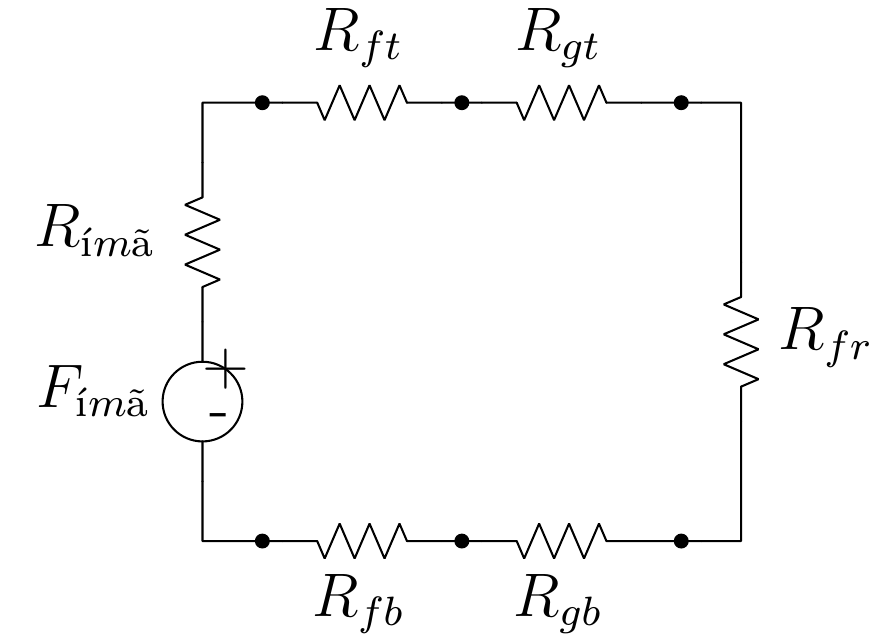
\includegraphics[width=0.4\linewidth]{Figs/circuito_passivo}
			\label{fig:circuito:passivo}
		}
		\hfill
		\subfigure[X and Y rotor displacement]{	
			\def\svgwidth{0.4\columnwidth}
			\includesvg{modelo_passivo_DxDy}
			\label{Fig:modelo:passivo:DxDz}
		}
		\caption{magnetic circuit of external stator and rotor }
	\end{figure}
	
	The magnetic field in the air gap (generated by the magnetics) can be decomposed into components $B_x$ and $B_z$ that are dependent on rotor displacement $\Delta_x$ and $\Delta_z$. The component z is responsible for stabilizing the passives degrees of freedom, the x component is a consequence of this topology causing the rotor instability on radial plane. Fig. \ref{Fig:modelo:passivo:DxDz} shows the magnetic flow on the external stator when displaced radially. 
			
	Magnetic attraction force calculated using the virtual work \citep{Chiba} principle been the equation quadratic to the magnetic field ($B(l)$) accumulated in air gap plus the area that it is concentrated ($S(l)$) divided by two times the air permeability ($\mu_0$).
	
	\begin{equation}
			F = \frac{B(l)^2 \, S(l)}{2 \mu_0}
	\end{equation}
	
	
	Both $B$ and $S$ are dependent of the air length ($l$), which makes the  attraction force non-linear.	Aiming the linearisation of the attractive force, the outer stator is project to work magnetic saturated making the quadratic portion of the equation constant ($B(l)^2 = cnt$) for variations on gap length. Besides linearisation, is possible with this technique obtain a higher axial stiffness without a large increase in radial stiffness, which would require higher energy to stabilize actives degree of freedom. In order to make the tilt passive stable, the force generated in $F_z$ must be superior to $F_x $ for a predefined angle range otherwise the tilt would cause a non symmetric force on the rotor causing it to get unstable.
	
	By the development of an analytical model it was possible to choose initial construction parameters for this proposed topology and then an finite element model was created to develop and verify the topology. The aim of this step is to get a good axial rigidity ($F_z$) with a small  radial force ($F_x$). Fig. \ref{fig:forca:passivo:fx} the result of rotor when subjected to radial displacement, it is remarkable the linear force resulted from this topology, by the other side, we have a non linear attraction force for axial displacement (\ref{fig:forca:passivo:comsol:dy}).
	
	% found that the force has a component different from zero when the rotor is aligned with the external stator (z = 0), this is caused by numeric errors on the FEM analysis. The achieved magnetic stiffness force for the axial displacement is of 20 kN/m and for the radial is of 60 kN/m. 

	
	\begin{figure}[ht]
		\subfigure[3D map of attraction force on the radial direction due to passive bearing system]{	
			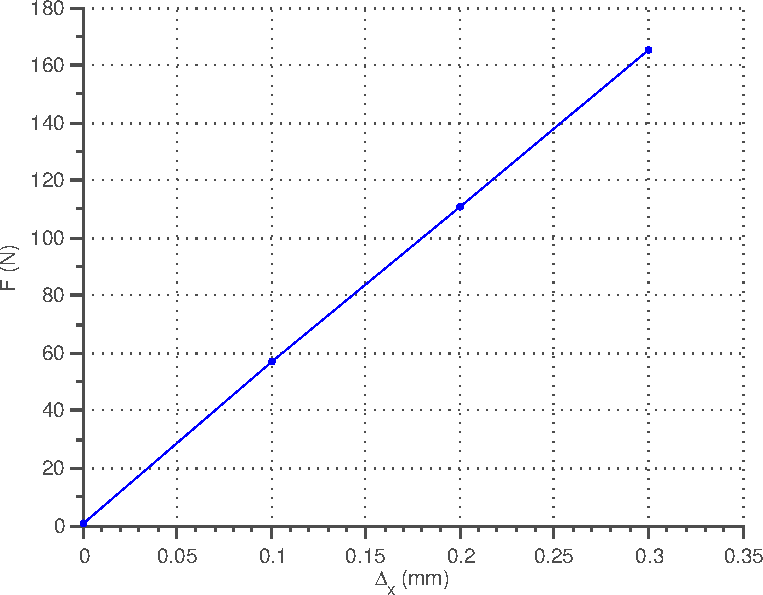
\includegraphics[width=0.5\linewidth]{./Figs/Simulacoes/Passivo/forca_passivo_comsol_fx}
			\label{fig:forca:passivo:fx}
		}
		\hfill
		\subfigure[X and Y rotor displacement]{	
			%{\textit{Magnetic Force (N) x Displacement Y (mm): Equilibrium point}}\\
			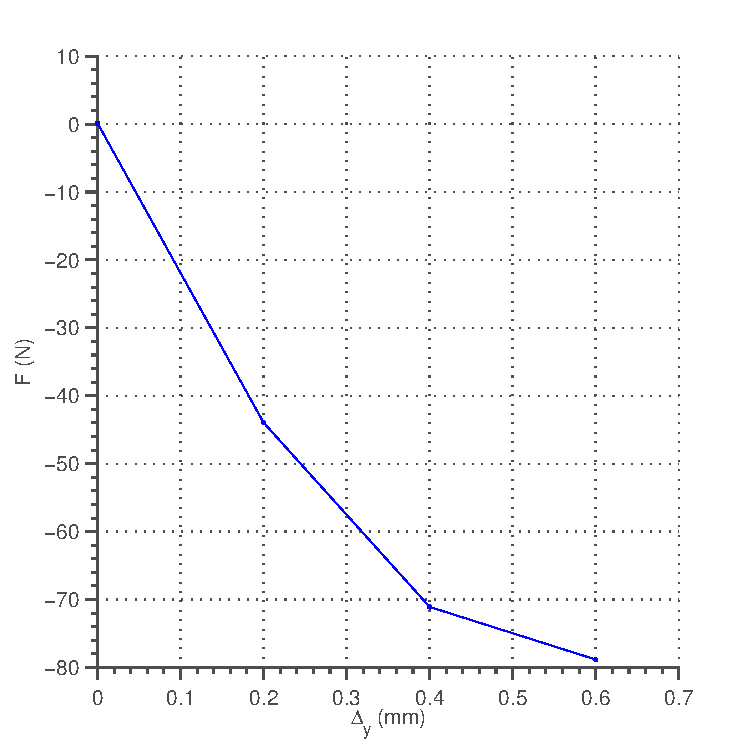
\includegraphics[width=0.45\linewidth]{./Figs/Simulacoes/Passivo/forca_passivo_comsol_dy}
			\label{fig:forca:passivo:comsol:dy}
		}
		\caption{Attraction force due to the passive circuit}
		\label{fig:forca:passivo}
	\end{figure}	
	
%	Is possible to write the attraction force on the radial axis as :
%	
%	\begin{equation}
%		F_p(x) = K_p x = 60k \, x
%	\end{equation}		
	
	\subsection{Inner stator and Rotor}
	
	The inner stator contains eight magnetic poles evenly distributed at 45 degrees, connected by a internal circulation ring. The poles act as electromagnet generating attraction force to stabilize the rotor on the radial direction (x, y). Each trio of poles acts as a single actuator
	, forcing the flux to cycles on a specific place maximizing the attraction force on the desired axis.
	
	Figure \ref{fig:modelo:mancal:estator:interno:fluxo} shows the internal stator with three poles acting as a single actuator: (A), (B), (C) and the respective magnetic flow generated by a current applied on the coils. Poles (A) and (C) work with inverse polarity of (B) forcing all flow over (B) and not by any other pole, thus maximizing the force of attraction $F_B$. The applied current on (A) and (C) is half the current in the main pole (B) preventing saturation.	Forces $F_A$ and $F_C$  have components in both directions x and y, for small changes, the components in the y direction is canceled ($F_y$). Leading to a single force in the x direction ($F_x$) :
	
	
	\begin{align}
		\vec{F}_x &= \vec{F}_B + \cos(45) (\vec{F}_{A} + \vec{F}_{C}) \label{eq:ativo:F:resultante:y} \\
		\vec{F}_y &=  \cos(45) (\vec{F}_{A} - \vec{F}_{C}) = 0 \label{eq:ativo:F:resultante:x}
	\end{align}	
	

	
	\begin{figure}[ht]
		\centering
		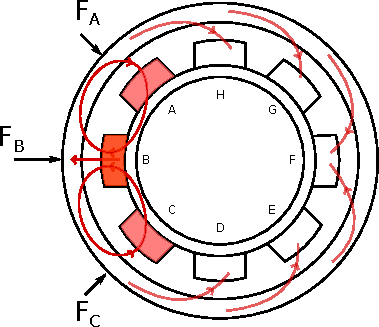
\includegraphics[width=0.6\linewidth]{./Figs/modelo_mancal_estator_interno_fluxo}
		\caption{Magnetic flux of active bearing system where A to H are the inner stator poles}
		\label{fig:modelo:mancal:estator:interno:fluxo}
	\end{figure}
	
	The magnetic circuit between the inner stator and the rotor can be split on four main elements: Coil magnetic field generating source, air gap reluctances which depends on the distance between the rotor poles and,  iron of the rotor and return ring
	
	The initial geometric parameters of the internal stator were raised by analyzing the power restriction. The maximum power for the system is 100W with a  supply voltage of 24V, resulting in a 4A max current. This electric current must be sufficient to generate an attraction force capable
	of compensate generated force created by passive circuit  in the largest  possible gap (Fig. \ref{fig:forca:passivo:fx}). From an analytic magnetic force model (Eq. \eqref{eq:ativo:F:resultante:y}) was possible to find a initial set of parameters (which include: areas, coil turns and air gap) able to generate a restorative force on the rotor with the imposed power restrictions. With a refined finite element model was possible to determine a better set of parameters by removing the unwanted saturated zones and maximizing the magnetic field on the gap by increasing the pole area. 
	
	Figure \ref{fig:forca:ativo} shows the achieved attraction force due the inner stator poles, this actuator has different gain depending on rotor position ($d_x$), larger the gap (negative dx) smaller the attraction force generated by the same current.
	
		
	\begin{figure}[ht]
	\centering
	\includegraphics[width=0.7\linewidth]{/Simulacoes/Ativo/mapa_forcas_ativo_comsol}
	\caption{Achieved attraction force on active circuit}
	\label{fig:forca:ativo}
	\end{figure}		
	
	%This model is used to 
	%\todo[inline]{comentar o impacto dessa nao linearidade do atuador}
	%\todo[inline]{gerar grafico de forca x deslocamento}
	
	
	\subsubsection{Inductance} \label{subsec:at:indutancia}
	
	Inductance plays a crucial role in the performance of the actuator and the main factor for its dynamic its is correlated with the generation capacity (magnetic) each pole and its current. Increasing the magnetic efficiency (with respect to applied current) of the poles impacts on a better attraction force but generates a higher inductance that is a worst actuator (in terms of dynamic response). For the present topology, the achieved inductance for each coils is of $56 mH$ with an electrical resistance of $4 \Omega$. 
	
	
	\subsection{Auxiliary Bearing}
	
	Auxiliary bearings are essential in any magnetic bearing, prevents the shock between the rotor and any critical part when the active control is disabled. The proposed auxiliary bearing is a solid ring of bronze limiting the maximum rotor excursion.
	
	\subsection{Bearing dimensions}
	
	The magnetic bearing has an external radius of 75.8 mm and max height of 18.0 mm. The nominal air length between the rotor and the external stator is of 1.2 mm and of 0.6 mm internal stator. 
	
	\section{Dynamic Model}
	
	%Via Lagrangian formalism we obtain the portion of the kinetic energy (T) from the rotor that results from the rotation of the rotor and it displacement. The potential energy (V) is due to axial translation of the rotor (in an environment with gravity): 
	
%	\subsection{Rotor Dynamic}
	
	Main rotor dynamics are basically influenced by your rotation speed ($\dot{\theta}$), inertia ($I$), mass ($m$) and its position ($x,y,z$) composing all the kinetic energy (T). The potential energy (V) is due to axial translation (z), gravity (g) and by the passive bearing stiffness ($K_z$) shown in Fig. \ref{fig:forca:passivo:comsol:dy} : 
	
	\begin{align}
		T_{\theta, x, y, z} &= \frac{1}{2} I_z \, \dot{\theta}^2 + \frac{1}{2} \, m \, \left( \dot{x}^2 + \dot{y}^2 + \dot{z}^2 \right) \notag \\
		V_z &= m \, g \, z + \frac{1}{2} \, K_z \, z^2
	\end{align}	

	Two different forces acts on the rotor: the  non-conservative forces ($Q^{nc}$) caused by the force applied by the actuators ($F_b$) that are depended on the rotor position and on the applied current ($i$); Conservative ($Q^{c}$) forces (which depend only on the position of the rotor) resulted from the passive attraction force ($K_p$). Both $F_b$ and $K_p$ are raised from the calculated force by finite element model, respectively shown on Fig. \ref{fig:forca:ativo} and Fig. \ref{fig:forca:passivo:fx}.

	\begin{align}
		Q_y^{nc} &= F_{by}(x,i)  \\
		Q_x^{nc} &= F_{bx}(y,i)  \\
		Q^{c}_x  &= K_p \, x \\
		Q^{c}_y  &= K_p \, y 
	\end{align}
	
	Differential dynamic model can be found by applying the Lagrange formalism on previews equations, resulting on the fallowing model:
			
	\begin{align}
		I \ddot{\theta} &= 0 \\
		m \ddot{x}		&= K_p \, x  - F_{bx}(x,i) \\
		m \ddot{y}		&= K_p \, y  - F_{by}(y,i)\\	
		m \ddot{z}  	&= K_z z + m g  + F_{pz}(z)
	\end{align}
	
	Theses equations shows an uncoupled system (considering balanced). Both x and y directions must be active controlled by $F_b$ to overcome the attractive force ($K_p$) generated to stabilize the z direction. 
	
	
%	\subsection{Actuator Dynamic}
		
	Actuator dynamics is primarily caused by coil's electrical resistance (R) and inductance dependent on the operation point (L(x,y)). At the operation point, the resulted actuator has cut-off frequency of $11Hz$. The actuator dynamic ($G_a(S)$) is :
	
	\begin{align}
		G_a(s) = \frac{1}{L(x,y) \, s + R} 
	\end{align}
	
	
	%\subsection{Block Diagram}
	
	Magnetic bearing radial dynamic modem can be represented by the block diagram on Fig. \ref{fig:diagrama_blocos_modelo_linear}. A controller ($C(s)$) is needed to stabilities the system controlling the current on actuators ($i$), this controller is project to work as regulatory ($R=0$).
	
	\begin{figure}[ht]
	\centering
	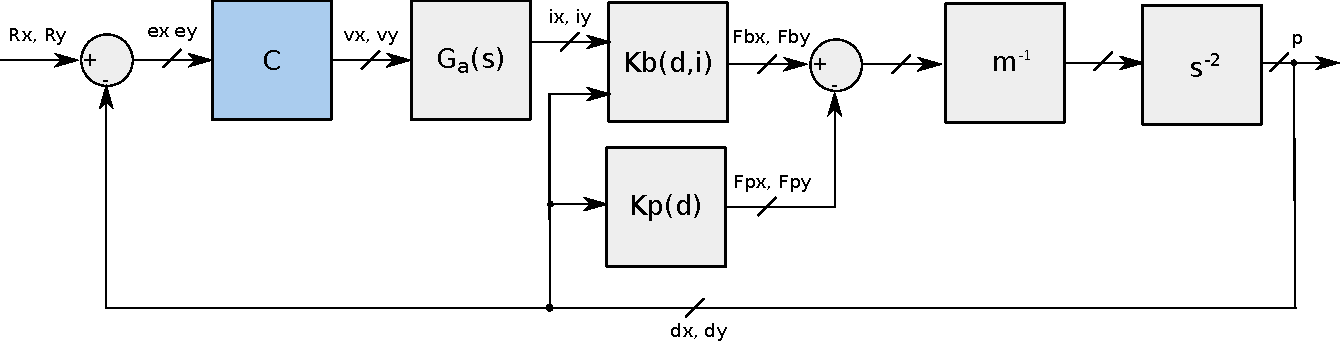
\includegraphics[width=1\linewidth]{Figs/Modelagem/diagrama_blocos_modelo_linear}
	\caption{Closed loop block diagram of radial rotor dynamic}
	\label{fig:diagrama_blocos_modelo_linear}
	\end{figure}	
	
	\section{CONTROLLER}
	
	Actuator gain ($Kb(d,i)$) is non linear and dependent of rotor position. To overcome this challenge a force control is designed instead of a current controller. The calculated force is applied to an estimator in order to calculate the current based on the request force and rotor position, Fig. \ref{fig:diagrama_controlador_estimador} is the proposed control scheme.
	
	%discarding the attractive force of the coils. he resulting control force is applied to an estimator, responsible for translating the desired strength in a voltage applied to the coils. This system dynamics can be model as:
	%\begin{equation}
	%G_p(s) = \frac{1}{m \, s^2 - K_p} = \frac{1}{0.369 \, s^2 - 60 \,E3}
	%\end{equation}
	
	\begin{figure}[ht]
	\centering
	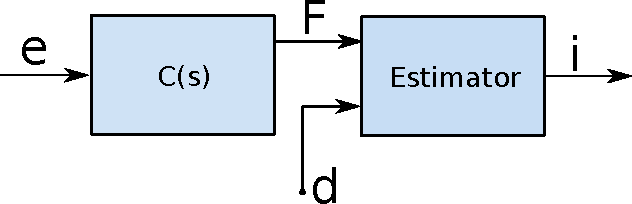
\includegraphics[width=0.3\linewidth]{Figs/Modelagem/controlador_estimador}
	\caption{Proposed controller scheme with current estimator}
	\label{fig:diagrama_controlador_estimador}
	\end{figure}
	
	This estimator block is implemented by simplified analytic model, that considerate the  air ($R_g$) reluctance as principal on the magnetic flux ($\phi$) circuit. The estimator is than dependent of applied current ($I$) , air gap length ($l_g$) and area ($S_g$). By the magnetic attraction force ($F$), we can derive the equation that correlates a current by de desired force.

	\begin{equation}
		I = \sqrt{\frac{2 \, F \, \mu_0}{S_g}} \, \frac{\mu_0 \, S_g^2}{n}
	\end{equation}
	
	A SISO loop-shaping controller ($H_{\infty}$) was project to model the system frequency response to be a first order low pass filter with cut-off-frequency of $100 Hz$ and a DC gain of 100. Frequency response of open loop and closed loop  is shown on Fig. \ref{fig:bode}.
	
	
	\begin{figure}[ht]
		\subfigure[Open loop]{	
			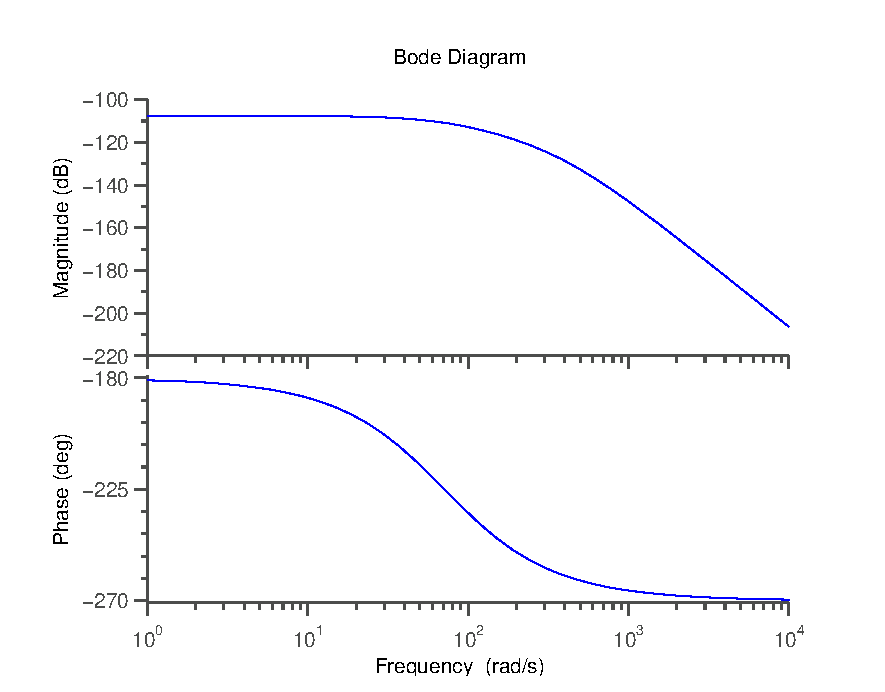
\includegraphics[width=0.5\linewidth]{./Figs/Modelagem/openloop.eps}
			\label{fig:bode:gs}
		}
		\hfill
		\subfigure[Closed loop with proposed controller]{	
			%{\textit{Magnetic Force (N) x Displacement Y (mm): Equilibrium point}}\\
			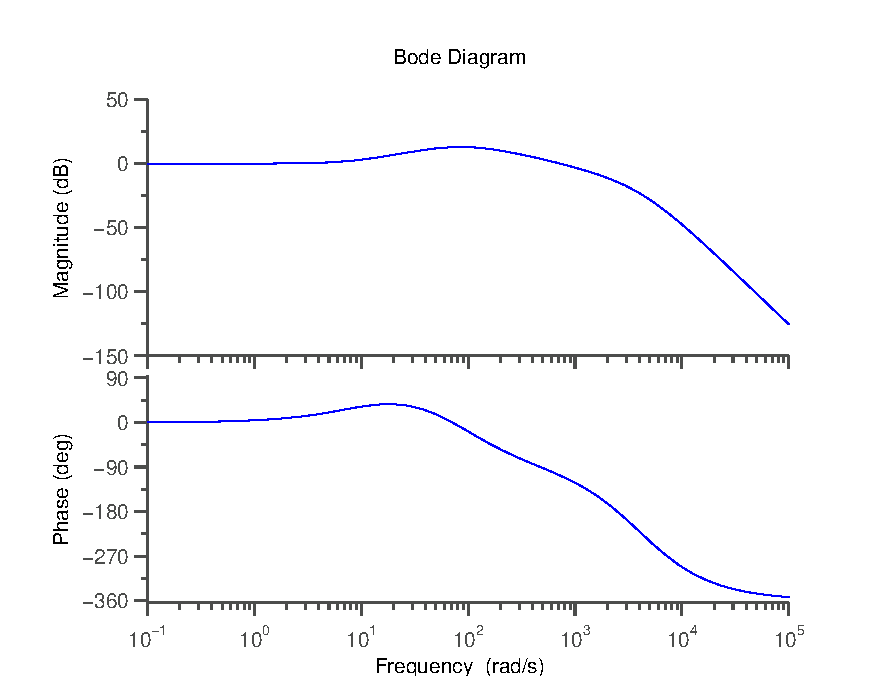
\includegraphics[width=0.5\linewidth]{./Figs/Modelagem/controlled.eps}
			\label{fig:bode:c}
		}
		\caption{Frequency response of open loop and controlled system}
		\label{fig:bode}
	\end{figure}	
	
	\section{CONCLUSION}
	
	In this paper, we proposed a new topology to a magnetic bearing system to a satellite reaction wheel. This bearing works radially active controlled by an eight electromagnets that exercises attraction force on the rotor. The passives degrees of freedom are stabilized due to a magnetic placed on the external stator. Optimizations and simulations were performed in order to achieve a bearing which complies with the restrictions, by the force models we project a dynamic model that represent the instable bearing part. A robust loopshaping controller is proposed to stabilize the rotor at it operation point, with little oscillation.
		
	\section{ACKNOWLEDGEMENTS}
	
	The author thanks to Instituto Mau\'{a} de Tecnologia and Dr. Leonardo Pinheiro that made this project possible.
	
	\section{REFERENCES} 
	
	\bibliographystyle{cobem2015}
	\renewcommand{\refname}{}
	\bibliography{./bibfile}
	
	\section{RESPONSIBILITY NOTICE}
	
	The authors are the only responsible for the printed material included in this paper.
	
\end{document}

